\documentclass[11pt,openany]{article}

\usepackage{amsfonts}
\usepackage{dsfont}
\usepackage{amssymb}
\usepackage{graphicx}
\usepackage{subcaption}
\usepackage{titlesec}
\usepackage{appendix}
\usepackage{amsmath}
\usepackage{pgfplots}
\usepackage{tikz}
\usepackage{stmaryrd}
\usepackage{circuitikz}
\usepackage{cancel}
\usepackage{slashed}
\usepackage{appendix}
\usepackage{hyperref}
\usepackage{siunitx}
\usepackage{url}
\usepackage[most]{tcolorbox}
\usepackage[margin=0.7in]{geometry}
\usepackage[compat=1.1.0]{tikz-feynman}
\usepackage[overload]{empheq}
\usepackage{braket}
\usepackage{mathtools}
\usepackage{float}
\usepackage{lineno}
\usepackage{xargs}
\usepackage{svg}


% better underbrace ==============================================

\usetikzlibrary{decorations.pathreplacing}
\makeatletter
\def\underbrace#1{%
	\@ifnextchar_{\tikz@@underbrace{#1}}{\tikz@@underbrace{#1}_{}}}
\def\tikz@@underbrace#1_#2{%
	\tikz[baseline=(a.base)] {\node[inner sep=0] (a) {\(\displaystyle #1\)};
		\draw[line cap=round,decorate,decoration={brace,amplitude=5pt}]
		(a.south east) -- node[below,inner sep=7pt] {\(\scriptstyle #2\)} (a.south west);}}
\def\overbrace#1{%
	\@ifnextchar^{\tikz@@overbrace{#1}}{\tikz@@overbrace{#1}^{}}}
\def\tikz@@overbrace#1^#2{%
	\tikz[baseline=(a.base)] {\node[inner sep=0] (a) {\(#1\)};
		\draw[line cap=round,decorate,decoration={brace,amplitude=5pt}]
		(a.north west) -- node[pos=.5,above,inner sep=7pt] {\(\scriptstyle #2\)} (a.north east);}}
\makeatother


% color box ==============================================================
\usepackage{xcolor}

% Syntax: \colorboxed[<color model>]{<color specification>}{<math formula>}
\newcommand*{\colorboxed}{}
\def\colorboxed#1#{%
	\colorboxedAux{#1}%
}
\newcommand*{\colorboxedAux}[3]{%
	% #1: optional argument for color model
	% #2: color specification
	% #3: formula
	\begingroup
	\colorlet{cb@saved}{.}%
	\color#1{#2}%
	\boxed{%
		\color{cb@saved}%
		#3%
	}%
	\endgroup
}

% miscellaneous commands

\newcommand{\dd}[2]{\frac{\mathrm{d}#1}{\mathrm{d}#2}}
\newcommand{\dpart}[2]{\frac{\partial#1}{\partial#2}}
\newcommandx{\intg}[4][2=,3=,4=]{\int\IfValueT{#3}{_{#3}}\IfValueT{#4}{^{#4}}\mathrm{d}\IfValueT{#2}{^{#2}}#1\hspace{1mm}}
\newcommand{\feynint}[1]{\int\frac{\mathrm{d}^D#1}{\left(2\pi\right)^D}}
\newcommand{\LL}{\mathrm{L}}
\newcommand{\RR}{\mathrm{R}}

\setlength\parindent{0pt}

\title{The Transverse Ising Model }
\author{Mathieu Ferey}

\addbibresource{biblio.bib}


\begin{document}
	
\begin{titlepage}
    
    \begin{center}
        ETH Zürich
        
        \vspace{1cm}

        \Huge
        \textbf{Quantum Simulations\\\huge of Gauge Theories\\}
        
        \vspace{1.5cm}

        \Large
        High Energy Physics Master Program\\
        Mathieu FEREY 
        
        \begin{figure}[h]
            \centering 
            
\includegraphics[scale=0.2]{Images/hep-logo.png}
        \end{figure}
        
        \rule{13cm}{0.5mm}
        \huge
        \textbf{\\Pure $\mathds{Z}_2$ Gauge Theory\\}
        \vspace{2mm}
        \Large
        \textbf{and the Transverse Field Ising Model\\}
        \rule{13cm}{0.5mm}
        
        \vspace{5mm}
        Herbstsemester 2023
        
        \vspace{1cm}
        
        \begin{figure}[h]
            \centering
            
\includegraphics[width=0.5\textwidth]{Images/eth_logo.png}
        \end{figure}
    
    	\vfill
    	
	    \large
		\underline{Lecturers}
	
		\vspace{1mm}
		Prof. Dr. Marina Krstic Marinkovic\\
		Dr. Joao Carlos Pinto Barros\\
		
		\vspace{1cm}
        \small
        Institut für Theoretische Physik\\
        ETH Zürich\\
        

    \end{center}


\end{titlepage}

\tableofcontents\clearpage

\section{Introduction}

Particle physicists started to develop Quantum Field Theory on the lattice as a mean to perform non-perturbative computations. This proved particularly useful in Quantum Chromodynamics, in which perturbation theory breaks down at low energy due to the running of the constant. The lattice formulation of gauge theories more generally allows for remarkable analogies with statistical physics. In particular, it has been shown that a $\mathds{Z}_2$ gauge theory on a two dimensional lattice exhibits phase transitions \cite{Wegner}. Furthermore, there exits a duality relation between this gauge theory and the Ising model in a transverse field, making clearer the analogy with statistical mechanics. If there exits an analytical solution for this quantum Ising model in one dimension, its two dimensional counterparts appears to be trickier. Fortunately, it can be mapped to a classical Ising model with an additional dimension sharing the same critical behaviour, allowing for a classical Monte-Carlo simulation. We have implemented it in Python. You can have a look at the $\mathrm{Display\_Notebook.ipynb}$ file in the Github repository \url{https://github.com/MathieuFerey/Transerve-Ising-Model}.

\section{Theoretical background}

\subsection{The $\mathds{Z}_2$ gauge theory and its Quantum Ising dual}

The Ising gauge theory with a discrete $\mathds{Z}_2$ gauge symmetry in $2+1$-dimensions \cite{fradkin} reads

\begin{equation}
	H_{\mathds{Z}_2} = -g\sum_{\vec{x},j}\sigma^x_j(\vec{x}) - \frac{1}{g}\sum_{\vec{x}}\sigma_1^z(\vec{x})\sigma_2^z(\vec{x}+e_1)\sigma_1^z(\vec{x}+e_2)\sigma_2^z(\vec{x}),
\end{equation}

where $\vec{x}$ refers to a position on the lattice, $j=1,2$ the two possible directions of a link, $\sigma_j^{x/z}(\vec{x})$ are the Pauli matrices, living on the links of the lattice. The local operator

\begin{equation}
	Q(\vec{x}) \equiv \sigma_1^x(\vec{x})\sigma_1^x(\vec{x}-e_1)\sigma_2^x(\vec{x})\sigma_2^x(\vec{x}-e_2)
\end{equation}

commutes with $H_{\mathds{Z}_2}$. It generates local gauge transformations. One can check that $Q^2=\mathds{1}$, so that the local symmetry of our problem is indeed $\mathds{Z}_2$. We define the gauge invariant operators

\begin{equation}
	\tau^z(\vec{r}) = \prod_{(\vec{x},j) \text{ pierced by } \tilde{\gamma}(\vec{r})}\sigma_j^x(\vec{x}),
\end{equation}

called the magnetic charge, as well as

\begin{equation}
	\tau^x(\vec{r}) = \prod_{(\vec{x},j) \text{ pierced by } \tilde{\gamma}(\vec{r})}\sigma_1^z(\vec{x})\sigma_2^z(\vec{x}+e_1)\sigma_1^z(\vec{x}+e_2)\sigma_2^z(\vec{x}),
\end{equation} 

the plaquette term. $\tilde{\gamma}$ is an open path on the dual lattice, which ends at position $\vec{r}$ on the dual lattice. The definitions of $\tau^z$ and $\tau^x$ are actually independent of the shape of $\tilde{\gamma}$. Since

\begin{equation}
	\left\{\tau_x(\vec{r}),\tau_z(\vec{r})\right\} = 0\text{ and }\tau_x^2(\vec{r}) = \tau_z^2(\vec{r}) = \mathds{1},
\end{equation} 

one can identify $\tau^x$ and $\tau^z$ as the Pauli matrices defined on  the dual lattice. 

\begin{figure}[H]
	\centering
	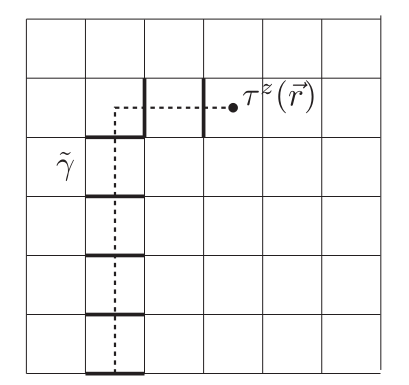
\includegraphics[width=0.3\textwidth]{Images/dual_lattice.png}
	\caption{The lattice and the path $\gamma$ used to defined operators on the dual lattice, from \cite{fradkin}.}
\end{figure}

One can check that the Hamiltonian on the dual lattice in terms of these operators reads

\begin{equation}
	H = -\sum_{i=1}^N\tau^z_i\tau^z_{i+1} - g\sum\tau^x_j,
\end{equation}

where $i,j$ run over the dual lattice sites. One recognizes the Ising model in a tranverse magnetic field (simply called the Transverse Ising Model, or the Quantum Ising Model) in two dimensions.


\subsection{The classical mapping of the Quantum Ising Model}

Our transverse Ising Model is not diagonal in the eigen-basis of $S^z$ and requires a quantum treatment. Luckily for us, a combination of clever tricks allows us to map the transverse field Ising Hamiltonian in $d$ dimensions to a classical anisotropic Ising Hamiltonian in $d+1$ dimensions \cite{Chakrabarti}. Let us demonstrate this in the case of the 1D Quantum Ising chain  for simplicity. Its Hamiltonian simply reads

\begin{equation}
	H = -J\sum_{i=1}^N S_i^zS_{i+1}^z - \Gamma\sum_{i=1}^N S_i^x.
\end{equation}

The thermodynamical properties of this system can all be derived through its partition function $Z = \mathrm{Tr}\exp(-\beta H)$, with $\beta=1/k_BT$. Everything starts with the Trotter formula \cite{trotter}:

\begin{equation}
	\exp\left(A_1+A_2\right) =  \lim_{M\to\infty}\left[\exp\left(A_1/M\right)\exp\left(A_2/M\right)\right]^M.
\end{equation}

Writing our Hamiltonian as $H = H_0 + V$, where $H_0$ is the spin-spin interaction and $V$ the action of the magnetic field, one can expand the partition function as follows (keeping the large $M$ limit implicit for shortness):

\begin{align*}
	Z &= \mathrm{Tr}e^{-\beta\left(H_0+V\right)}\\
	&= \mathrm{Tr}\left[e^{-\beta H_0/M}e^{-\beta V/M}\right]^M\\
	&= \sum_{\left\{S^1_1,\cdots,S^1_N\right\}}\bra{S^1_1,\cdots,S^1_N}e^{-\beta H_0/M}e^{-\beta V/M}\cdots\\
	&\hspace{3cm}\times e^{-\beta H_0/M}e^{-\beta V/M}\ket{S^1_1,\cdots,S^1_N},
\end{align*}

where $\ket{S_i^1} = \ket{\pm1}_i$ is an eigenstates of $S_i^z$. The sum runs over all possible configurations for the lattice. Now, between each pair of exponential we can insert the identity in the form

\begin{equation}
	\mathds{1} = \sum_{\left\{S^k_1,\cdots,S^k_N\right\}}\ket{S^k_1,\cdots,S^k_N}\bra{S^k_1,\cdots,S^k_N}.
\end{equation}

The $k$ index, which simply labels one complete set of eigenstates of $S_z$, can be regarded as an additional dimension to our lattice (often referred to as the Trotter dimension). The spin $S_i^k$ can be understood the spin living on the $(i,k)$ site of a 2 dimensional lattice. Then

\begin{equation}
	Z = \sum_{\left\{S\right\}}\prod_{k=1}^M\bra{S^k_1,\cdots,S^k_N}e^{-\beta H_0/M}e^{-\beta V/M}\ket{S^{k+1}_1,\cdots,S^{k+1}_N},
\end{equation}

where we introduced periodic boundary conditions in the Trotter dimension, $\ket{S^{M+1}_1,\cdots,S^{M+1}_N} = \ket{S^1_1,\cdots,S^1_N}$ so as to match the braket sandwiching of the trace. We have used the shorthand notation $\sum_{\left\{S\right\}} = \sum_{\left\{S_1^1,\cdots,S_N^1\right\}}\cdots\sum_{\left\{S_1^M,\cdots,S_N^M\right\}}$, which is just a sum over all possible configurations of our 2D lattice. Now, the $H_0$ exponential is diagonal in the $\ket{S^k_1,\cdots,S^k_N}$ basis, so that, using its hermiticity,

\begin{equation}
	\bra{S^k_1,\cdots,S^k_N}e^{-\beta H_0/M} = \exp\left[\frac{\beta J}{M}\sum_{i=1}^N S_i^k S_{i+1}^k\right]\bra{S^k_1,\cdots,S^k_N}.
\end{equation}

The second exponential now reads

\begin{align*}
	\bra{S^k_1,\cdots,S^k_N}e^{-\beta V/M}\ket{S^{k+1}_1,\cdots,S^{k+1}_N} &= \bra{S^k_1,\cdots,S^k_N}\exp\left[\frac{\beta\Gamma}{M}\sum_{i=1}^N S_i^x\right]\ket{S^{k+1}_1,\cdots,S^{k+1}_N}\\
	&= \prod_{i=1}^N\bra{S_i^k}e^{\beta\Gamma S_i^x/M}\ket{S_i^{k+1}}.
\end{align*}

Here comes a trick, keeping in mind that $S^x$ just flips the spin and that $(S^x)^2=\mathds{1}$:

\begin{align*}
	\bra{S}e^{aS^x}\ket{S'} &= \bra{S}\left(\sum_{n=0}^\infty\frac{a^{2n}(S^x)^{2n}}{n!} + \sum_{n=0}^\infty\frac{a^{2n+1}(S^x)^{2n+1}}{n!}\right)\ket{S'}\\
	&= \cosh{a}\braket{S,S'} + \sinh{a}\bra{S}S^x\ket{S'}\\
	&= \cosh{a}\braket{S,S'} + \sinh{a}\braket{S,-S'}\\
	&= \begin{cases}
		&\cosh{a} \text{ if } S=S',\\
		&\sinh{a} \text{ if } S=-S'.
	\end{cases}
\end{align*}

Now, we rewrite this matrix element using

\begin{align*}
	\left(\frac{1}{2}\sinh{2a}\right)^{1/2}\exp\left[\frac{SS'}{2}\ln\coth{a}\right] &= \sqrt{\sinh{a}\cosh{a}}\times
		\begin{cases}
			&\exp\left[\dfrac{1}{2}\ln\coth{a}\right] \text{ if } S=S'			\vspace{1mm}\\
			&\exp\left[-\dfrac{1}{2}\ln\coth{a}\right] \text{ if } S=-S'
		\end{cases}\\
	& = \sqrt{\sinh{a}\cosh{a}}\times
	\begin{cases}
		&\sqrt{\cosh{a}/\sinh{a}} \text{ if } S=S'\\
		&\sqrt{\sinh{a}/\cosh{a}} \text{ if } S=-S'
	\end{cases}\\
	&= \begin{cases}
		&\cosh{a} \text{ if } S=S'\\
		&\sinh{a} \text{ if } S=-S'
	\end{cases}\\
	&= \bra{S}e^{aS^x}\ket{S'}
\end{align*}

This was a long road, but we can finally put everything together.

\begin{align*}
	Z &= \sum_{\left\{S\right\}}\prod_{k=1}^M\prod_{i=1}^N\exp\left[\frac{\beta J}{M}S_i^kS_{i+1}^k\right]\left(\frac{1}{2}\sinh{2\beta\Gamma/M}\right)^{1/2}\exp\left[\frac{S_i^kS_i^{k+1}}{2}\ln\coth(\beta\Gamma/M)\right]\\
	&= \left(\frac{1}{2}\sinh(2\beta\Gamma/M)\right)^{MN/2}\sum_{\left\{S\right\}}\exp\left[-\frac{\beta}{M}\left(-J\sum_{i=1}^N\sum_{k=1}^M S_i^k S_{i+1}^k - \frac{M}{2\beta}\ln\coth\left(\dfrac{\beta\Gamma}{M}\right)\sum_{i=1}^N\sum_{k=1}^M S_i^k S_i^{k+1}\right)\right]\\
	&= C\hspace{1mm}\mathrm{Tr}\left[e^{-\beta_\mathrm{cl}H_\mathrm{eff}}\right],
\end{align*}

with the classical temperature $\beta_\mathrm{cl} = \beta/M$. Let us also abbreviate $K_M = \dfrac{1}{2\beta}\ln\coth\left(\dfrac{\beta\Gamma}{M}\right)$. In the large $M$ limit, the prefactor vanishes, so that it drops out of any physical observables (obtained by differentiating the logarithm of the partition function). One recognizes in $H_\mathrm{eff}$ the Hamiltonian of a classical (since the $S_i^k$ are just numbers) anisotropic Ising model without any magnetic field. The weird thing is that the coupling constant of the spin-spin interactions depend on the lattice size in the  Trotter dimension and even on the temperature for the interactions along the Trotter dimension. The quantum Ising model dual to our $\mathds{Z}_2$ gauge Hamiltonian is two dimensional, the above result therefore needs to be generalized to higher dimensions. The quantum Ising model on a two dimensional $N_x\times N_y$ lattice

\begin{equation}
	H = -J\sum_{i,j}S^z_{i,j}\left(S^z_{i+1,j} + S^z_{i,j+1}\right) -\Gamma\sum_{i,j}S^x_{i,j},
\end{equation}

can be mapped to the 3D classical anisotropic Ising model on a $N_x\times N_y \times N_z$ lattice

\begin{equation}
	H_\mathrm{eff} = -\sum_{k=1}^{N_z}\sum_{i,j}\left[J S_{i,j,k}\left(S_{i+1,j,k} + S_{i,j+1,k}\right) + K_{N_z} S_{i,j,k}S_{i,j,k+1}\right]
\end{equation}


\subsection{Phase transition}

Let us look into some thermodynamical properties of the system. One defines the magnetisation per spin as

\begin{equation}
	m = \frac{1}{N}\sum_\mathrm{i,j,k}S_{i,j,k},
\end{equation}

where $N=N_xN_yN_z$ is the total number of spins. Thanks to our Monte-Carlo algorithm, we will be able to estimate its average

\begin{equation}
	\langle m\rangle = \frac{1}{N_\mathrm{samples}}\sum_\mathrm{samples} m_\mathrm{sample}.
\end{equation}

A nice observable is also the susceptibility of the system

\begin{equation}
	\chi = \dpart{m}{\Gamma} = \beta\left(\langle m^2\rangle - \langle m\rangle^2\right).
\end{equation}

It will prove particularly useful for probing phase transitions. The partition function of the $d+1$ classical Ising model reads $Z\propto\mathrm{Tr}\left[\exp\left(-\frac{\beta}{N_z}H_\mathrm{eff}\right)\right]$. Since $N_z\to\infty$, a thermal phase transition of the classical system at finite temperature $\beta_{\mathrm{cl}}=\beta/N_z$ should give rise to a phase transition at $T=0$ in the quantum system, namely a phase transition driven by quantum fluctuations rather than thermal fluctuations. In the $T=0$ limit, one can indeed expect two phases \cite{Vasseur}:

\begin{itemize}
	
	\item $\Gamma/J \ll 1$: the Hamiltonian is dominated by $\displaystyle-J\sum_{\langle i,j\rangle}S^z_iS^z_j$.
	
	We have two degenerate ground states, all spins up or all spins down. This is a ferromagnetic ordered phase, with domain wall excitations.
	
	\item $\Gamma/J \gg 1$: the Hamiltonian is dominated by $\displaystyle-\Gamma\sum_iS^x_i$.
	
	We have one ground state, where all spins are aligned with the magnetic field (each in a state $\frac{1}{\sqrt{2}}\left[\ket{\uparrow}+\ket{\downarrow}\right]$). This a paramagnetic disordered phase, with quasi-particle excitations (i.e. single spin flips).
	
\end{itemize}


\section{Metropolis-Hasting Monte-Carlo algorithm}

We have derived a classical Ising Hamiltonian which shares, up to a constant, the same partition function with the quantum model. We should therefore be able to study its thermodynamical properties, mainly its phase transitions, through a simple Monte-Carlo algorithm, which naively works as follows \cite{Binder}:

\begin{tcolorbox}[title=Metropolis-Hasting algorithm]
	
	\begin{enumerate}
		
		\item Start from an initial configuration.
		
		\item Sweep through the lattice. For as many spins as there are in the system, flip one randomly chosen spin on the lattice and compute the change in energy $\mathrm{d}E$.
			\begin{itemize}
				\item If $\mathrm{d}E<0$: accept this new configuration.
				
				\item Else: accept the configuration with probability $\exp\left(-\beta \mathrm{d}E\right)$, otherwise reject it.
			\end{itemize}
		
		During one sweep, we expect to have given most of the spins of the lattice a chance to flip. The configuration generated after one sweep is added to our sampling.
		
		\item Repeat the sweeps until the required number of configurations have been generated.
		
		\item Ditch the first $N_\mathrm{eq}$ configurations generated before reaching equilibrium.
		
	\end{enumerate}
	
\end{tcolorbox}

The Metropolis procedure was specifically designed to generate a sample configurations according to their probability distribution. One can then compute averages without worrying about computing the partition function of the system:

\begin{equation}
	\langle O\rangle = \frac{1}{N_\mathrm{samples}}\sum_\mathrm{samples} O_\mathrm{sample},
\end{equation}

with $O_\mathrm{sample}$ is the value of the observable $O$ for one sample generated by our Monte-Carlo procedure. A few subtleties have to be taken into account. The time taken by the Metropolis algorithm to reach equilibrium -that is to say the number of steps required to generate configurations with the proper probability distribution- is not easy to guess, and has to be adjusted "by hand" quite qualitatively. One can for example plot the evolution of desired observables as the Monte-Carlo sampling goes on. We can however expect typical behaviours.

\begin{itemize}
	
	\item The bigger the lattice, the more steps will be required to thoroughly explore the space of configurations (of which there are $2^{N_xN_yN_z}$!). This is troublesome in our case since the classical mapping only holds in the large $N_z$ limit. This can be partially solved by the means of cluster methods, where the Metropolis update consists of flipping whole chunks of spins at the same time. Computing the change in energy will however naively requires going through the whole lattice, with complexity $\mathcal{O}\left(N_xN_yN_z\right)$, which might be too costly for thousands of Metropolis updates.
	
	\item One as to choose a suitable initial configuration so as to minimize the equilibration time. Starting from a completely random configuration is not very smart when looking at ordered phases (for example at low temperature), since randomness mimics very high temperature behaviour. When looking at the evolution of a quantity with temperature, one can start at low temperature from a very ordered system (say all spins up), and use the last configuration generated when dealing with the next temperature point. We can expect this configuration to be rather close to equilibrium, and therefore spare costly equilibration time.
	
\end{itemize}


\section{Results}

We have implemented the Monte-Carlo algorithm in a Notebook submitted with this report. Let us first look at the evolution of our Monte-Carlo process starting from a completely random configuration (Figure \ref{fig:MC}).  A hundred of steps seem to be enough to reach equilibrium and oscillate around it.

\begin{figure}[H]
	\centering
	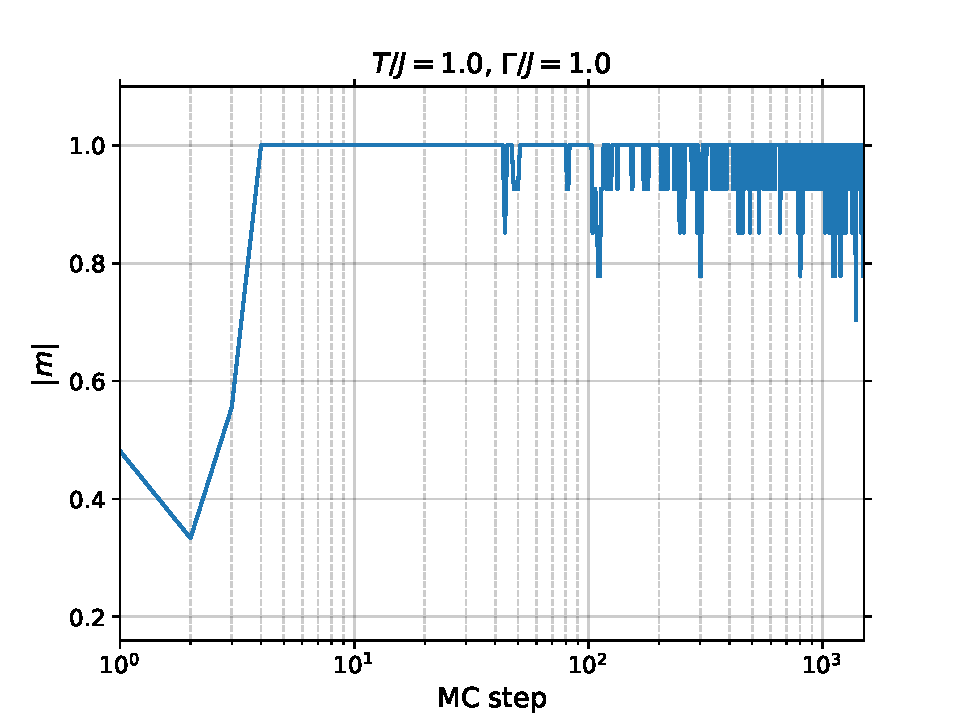
\includegraphics[width=0.5\textwidth]{Plots/MC.pdf}
	\caption{Magnetisation per spin as our Monte-Carlo process goes on at $T/J=1$ and $\Gamma/J=1$ for a $3\times3\times3$ lattice. One MC step represents a whole sweep of the lattice.}
	\label{fig:MC}
\end{figure}

We can now look at the evolution of magnetization with temperature and transverse field strength $\Gamma$. Our Monte-Carlo algorithm is quite slow, so that the $N_z\to \infty$ limit is worrying. The magnetic susceptibility of our system for different values of $N_z$ is displayed in Figure \ref{fig:transition_chi_nz}. A larger Trotter dimension makes the temperature phase transition sharper, as expected for finite-size systems. The value of the critical temperature does not seem to greatly change with $N_z$, so that sticking to small Trotter dimension will be sufficient to respect our classical mapping.

\begin{figure}[H]
	\centering
	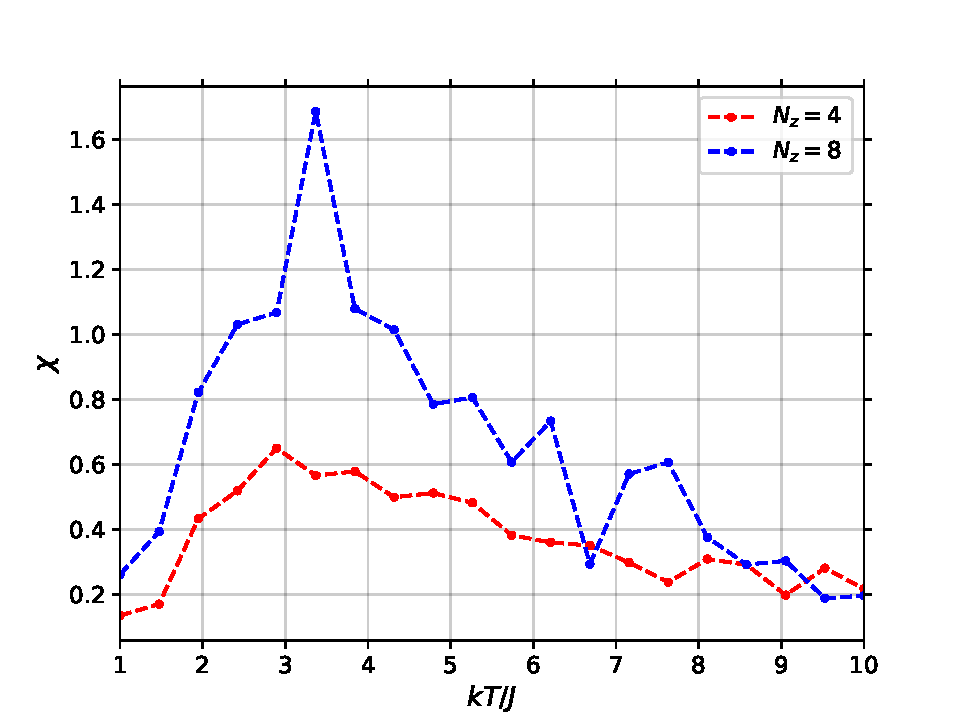
\includegraphics[width=0.5\textwidth]{Plots/T_transition_chi_nz.pdf}
	\caption{Susceptibility as a function of temperature for $\Gamma/J=1$ for a $2\times2\times N_z$ lattice.}
	\label{fig:transition_chi_nz}
\end{figure}

Figure \ref{fig:T_transition} displays a thermal phase transition.
 
\begin{figure}[H]
	\centering
	\begin{subfigure}{0.45\textwidth}
		\centering
		\caption{}
		\label{fig:T_m}
		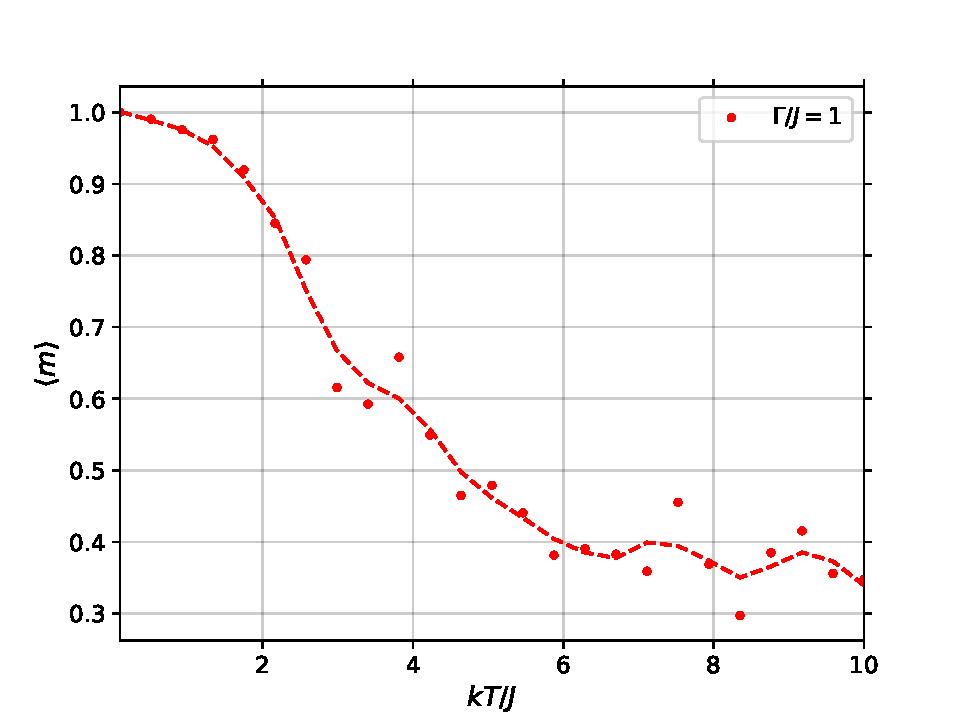
\includegraphics[width=\textwidth]{Plots/T_transition_m.pdf}
	\end{subfigure}
	\begin{subfigure}{0.45\textwidth}
		\centering
		\caption{}
		\label{fig:T_chi}
		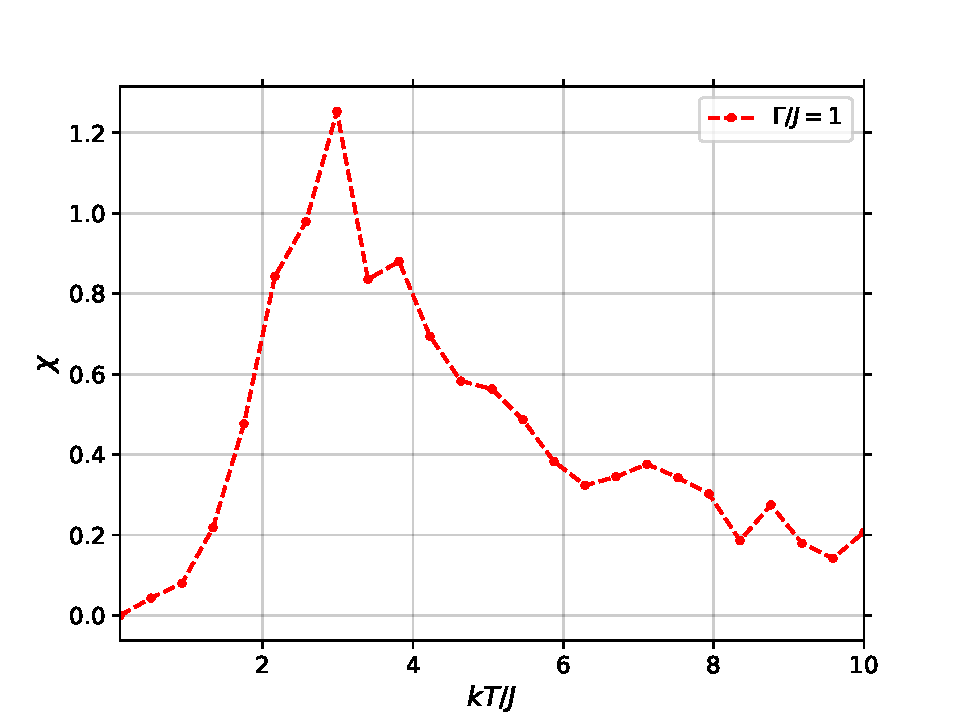
\includegraphics[width=\textwidth]{Plots/T_transition_chi.pdf}
	\end{subfigure}
	\caption{Average magnetisation per spin \ref{fig:T_m} and susceptibility \ref{fig:T_chi} as a function of the transverse field for a $3\times3\times4$ lattice at temperature $\Gamma/J=1$. The system clearly exhibits a phase transition between a ferromagnetic and paramagnetic phase.}
	\label{fig:T_transition}
\end{figure}

The real star of the show is of course $T=0$ phase transition, for which we want to compute magnetisation and susceptibility as a function of the field strength $\Gamma$. If there exists algorithms designed to analyze quantum system directly at $T=0$, such as Green's function Monte-Carlo, ours can only perform finite temperature computations. We can however simulate the system for decreasing values of $T$ and extrapolate the $T=0$ behaviour. This is displayed in Figure \ref{fig:gamma_transition_T}. The position of the transition does not seem to change as the temperature decreases. At very low temperatures, the interaction in the Trotter direction $ \frac{1}{2\beta}\ln\coth(\beta\Gamma/N_z)$ becomes singular and more Monte-Carlo steps in order to obtain neat looking curves. The algorithm is too slow to hope to approach even lower temperatures in a reasonable amount of time.

\begin{figure}[H]
	\centering
	\begin{subfigure}{0.45\textwidth}
		\centering
		\caption{}
		\label{fig:gamma_m_T}
		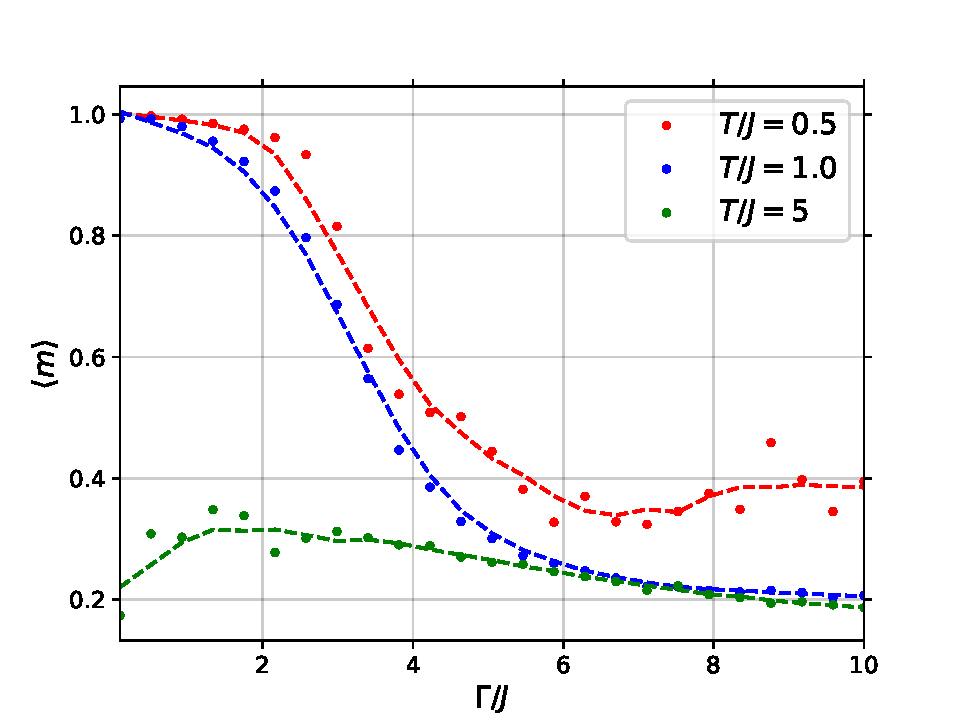
\includegraphics[width=\textwidth]{Plots/gamma_transition_m_T.pdf}
	\end{subfigure}
	\begin{subfigure}{0.45\textwidth}
		\centering
		\caption{}
		\label{fig:gamma_chi_T}
		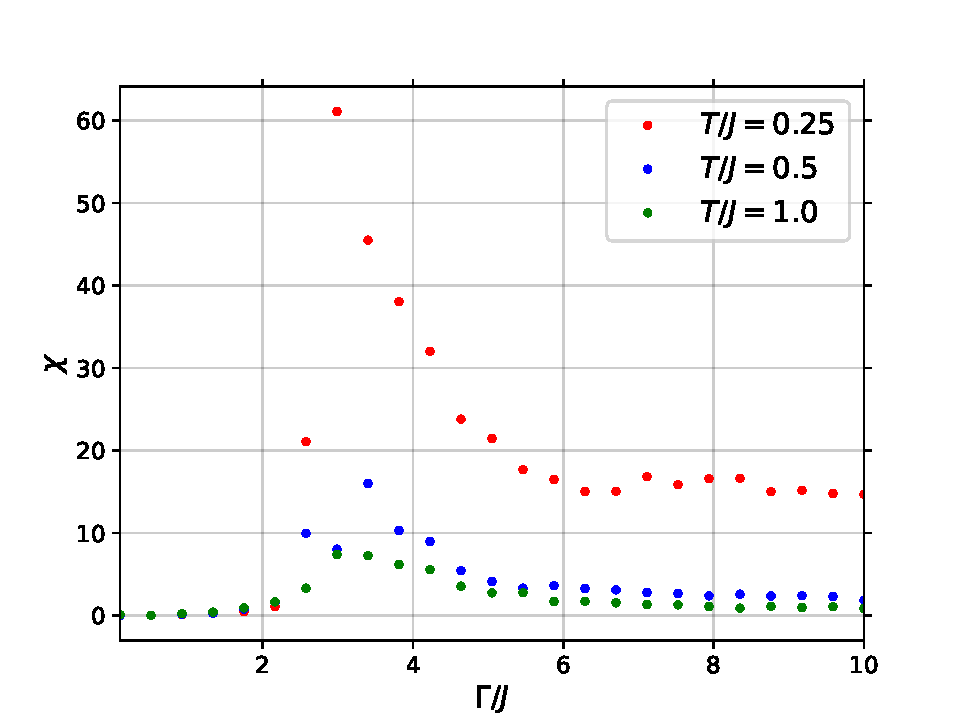
\includegraphics[width=\textwidth]{Plots/gamma_transition_chi_T.pdf}
	\end{subfigure}
	\caption{Average magnetisation per spin \ref{fig:gamma_m} and susceptibility \ref{fig:gamma_chi} as a function of the transverse field for a $4\times4\times10$ lattice at temperature three different temperatures. The system clearly exhibits a phase transition between a ferromagnetic and paramagnetic phase.}
	\label{fig:gamma_transition_T}
\end{figure}


\section{Closing remarks}

A system as simple as the transverse Ising model hides plethora of numerical and physical complexity, which are difficult to explore in so little time -especially for the high-energy physics student I am, who has forgotten most of his statistical physics lectures. If we managed to perform Monte-Carlo simulations and recover critical behaviours, the algorithm is too slow to conduct a very thorough investigation of the thermodynamical properties of the Quantum Ising Model -for example draw a full phase diagram such as in \cite{Chakrabarti}. The numerical difficulties arising from the diverging behaviour of the interaction in the Trotter direction at low temperature forbids a true analysis of the ground state of the transverse Ising model, and forbids any further comparison with its dual $\mathds{Z}_2$ gauge-theory, which has been investigated using exact diagonalisation by another student attending the course.


\clearpage\printbibliography

\end{document}